\chapter[Status in 2019]{Status of transboundary air pollution in 2019}
\label{ch:chapterStatus}

\old{TODO}

{\bf{Svetlana Tsyro, Wenche Aas, Sverre Solberg, Anna Benedictow, Hilde Fagerli and Thomas Scheuschner}}
\vspace{30pt}

This chapter describes the status of transboundary air pollution in 2018. A short summary of the meteorological conditions for 2018 is presented and the EMEP network of measurements in 2018 is briefly described. Thereafter, the status of air pollution and exceedances in 2018 is discussed.

The summer of 2018 was unusually warm and dry in large parts of Europe; therefore a separate chapter is devoted to the effect of these meteorological conditions on air pollution (Chapter \ref{ch:Summer2018}).

\section{Meteorological conditions in 2018}
\label{sec:meteo}
Air pollution is significantly influenced by both emissions and weather conditions. Temperature and precipitation are particularly important factors. A short summary describing the situation in 2018 with respect to these two parameters, based on model results and as reported by the meteorological institutes in European and EECCA countries, is given below.

The meteorological data to drive the EMEP MSC-W air quality model have been generated by the Integrated Forecast System (IFS) model of the European Centre for Medium-Range Weather Forecasts (ECMWF), hereafter referred to as the ECMWF-IFS model. In the meteorological community the ECMWF-IFS model is considered state-of-the-art, and MSC-W has been using this model in hindcast mode to generate meteorological reanalyses for the year to be studied. IFS Cycle 40r1 is the version used for the year 2018 model runs. In the following section, temperature and precipitation in 2018 are compared to the 2000-2017 average based on the same ECMWF-IFS model setup.

\subsection{Temperature and precipitation}
The mean temperature in 2018 was reported by the World Meteorological Organisation \citep{WMO1233:2018} as the fourth highest on record globally, and the third highest in Europe. In the Arctic, according to the Arctic Report Card 2018 \citep{Overland:ARC2018}, the period October 2017 to September 2018 was the second warmest 12-month period on record since 1900 (after 2015-2016).
Global precipitation anomalies in 2018 were also reported by the WMO \citep{WMO1233:2018} with above-average precipitation in south-west and south-east Europe, in contrast to rainfall deficits in central and northern Europe. 

\begin{figure*}[h]
  \centering
  \subfigure[$\Delta$temperature at 2m (2018-climavg)] {\includegraphics*[viewport=187 60 430 750,clip,angle=90,scale=0.65]{FIGS_STATUS/2018-2000_2017IFS_t2m_EMEP01.pdf}}
  \subfigure[$\Delta$precipitation (2018-climavg)] {\includegraphics*[viewport=187 60 430 750,clip,angle=90,scale=0.65]{FIGS_STATUS/2018-2000_2017IFS_aPr_EMEP01.pdf}}
  \caption{Meteorological conditions in 2018 compared to the 2000-2017 average (climavg) for: a) Annual mean temperature at 2m [K] and b) Annual precipitation [mm]. The meteorological data have been calculated with the ECMWF-IFS model.}
\label{fig:2018-avMET}
\end{figure*}

Compared to the 2000-2017 average, higher temperatures in 2018 are clearly seen in Figure~\ref{fig:2018-avMET} a) over the Arctic, central and south-eastern Europe, and slightly lower temperatures 
confined to limited parts of north-western and south-western Europe, Kazakhstan and southern Russia. Particularly, Turkey had abnormally high temperatures throughout the year with means above normal for all months \citep{Sensoy:Turkey2018}.
Svalbard recorded large positive temperature anomalies in 2018 \citep{Overland:ARC2018}, especially in the beginning with a record warm May and towards the end of the year.

Despite some local extreme precipitation events with heavy rainfall in short time, especially in western and south central Europe, 2018 was overall a dry year in much of Europe. Compared to the 2000-2017 average, precipitation in 2018  (Figure~\ref{fig:2018-avMET} b)) shows higher amounts than normal in south-west and south-east Europe, and below-normal precipitation in central and northern Europe. Iceland had more precipitation than the 2000-2017 average in 2018 with Reykjavik breaking a record with 261 rainy days.

\begin{figure}[h]
  \centering 
  \subfigure[$\Delta$temperature at 2m (AprSep 2018-climavg)]{\includegraphics*[viewport=187 60 425 750,clip,angle=90,scale=0.65]{FIGS_STATUS/2018-2000_2017IFS_halfYrSum_T2m.pdf}}
  \subfigure[$\Delta$temperature at 2m (OctMar 2017-climavg)]{\includegraphics*[viewport=187 60 425 750,clip,angle=90,scale=0.65]{FIGS_STATUS/2018-2000_2017IFS_halfYrVin_T2m.pdf}}
  \caption{Meteorological conditions in 2018 compared to the 2000-2017 average (climavg) for: a) Summer (April-September) temperature [K], b) Winter (January-March and October-December) temperature [K]. The meteorological data have been calculated with the ECMWF-IFS model.} 
\label{fig:temp2018-avMET}
\end{figure}

Figure~\ref{fig:temp2018-avMET} shows the temperatures in 2018 compared to the 2000-2017 average in Europe for the summer months (April through September) and the winter months (October through December and January through March). 
Characteristic of the year 2018 is the higher than average summer temperature in central Europe, as shown in Figure~\ref{fig:temp2018-avMET}~a) with temperatures in 2018 compared to the 2000-2017 average. The heat wave during the summer of 2018 and its effect on air pollution levels are discussed in more detail in a separate chapter (Chapter~\ref{ch:Summer2018}). Spring, with an exceptionally warm May, was the warmest on record in Bosnia and Herzegovina, Bulgaria, Greece, Serbia and Turkey. May was also the warmest month on record in Svalbard, Scandinavia, the Baltic countries, Austria and Germany. Many of these regions continued breaking temperature records in the summer and autumn months.
In Spain, the United Kingdom, Ireland and northern Scandinavia the winter was colder than normal, and close to normal in central Europe. Southeastern Europe experienced a milder than average winter, see Figure~\ref{fig:temp2018-avMET}~b). In February and March, easterly winds brought cold Siberian air to most countries in Europe. March was particularly cold in European parts of Russia with an anomaly of about -3$\degrees$C. In April the weather changed from winter to summer conditions in only a few days for some areas in central and southeastern Europe. 
Bosnia and Herzegovina and Serbia had their warmest October on record.

\begin{figure}[H]
  \centering
  \subfigure[$\Delta$precipitation (AprSep 2018-climavg)]{\includegraphics*[viewport=187 60 425 752,clip,angle=90,scale=0.65]{FIGS_STATUS/2018-2000_2017IFS_halfYrSum_APr.pdf}}
  \subfigure[$\Delta$precipitation (OctMar 2018-climavg)]{\includegraphics*[viewport=187 60 425 752,clip,angle=90,scale=0.65]{FIGS_STATUS/2018-2000_2017IFS_halfYrVin_APr.pdf}}
  \caption{Meteorological conditions in 2018 compared to the 2000-2017 average (climavg) for: a) Summer (April-September) precipitation [mm], b) winter (January-March and October-December) precipitation [mm]. The meteorological data have been calculated with the ECMWF-IFS model.} 
\label{fig:prec2017-avMET}
\end{figure}

Flooding affected central Europe in the beginning of the year, but the same area later experienced extremely dry conditions (see precipitation in winter and summer in 2018 compared to the 2000-2017 average in Figure~\ref{fig:prec2017-avMET}). Precipitation for April through September in Figure~\ref{fig:prec2017-avMET}~a) shows that northern and central Europe had much less precipitation than the 2000-2017 average, with the exception of northwestern coastal regions. Latvia reported its second driest spring, Ireland and the Netherlands its driest summer on record, and in Sweden a severe drought from May to July caused extensive forest fires in central parts of the country. Drought was also reported in the United Kingdom. Germany reported the second driest April-September period and Czechia its driest January-August period on record.
However, above-average precipitation amounts were observed in south-west and south-east Europe in both the summer and winter months. In Figure~\ref{fig:prec2017-avMET}~b) precipitation for the winter months (January-March and October-December) in 2018), compared to the 2000-2017 average, is higher than average in western, central and southern Europe, and lower than average in north-eastern Europe. With the cold conditions in late February and early March some areas in western and southern Europe (Ireland, France, Italy and Portugal) experienced abnormal conditions with snow and freezing rain. And the year ended with above-average precipitation in December for most of central Europe, terminating the drought of the previous two seasons.


\section{Measurement network 2018} 
\label{Obs_2018}

In 2018, a total of 35 Parties reported measurement data of inorganic components, particulate matter and/or ozone to EMEP from altogether 170 sites, which are the relevant components for level 1 sites \citep{MonStrat2019}. 
All the data are available from the EBAS database (\url{http://ebas.nilu.no/}) and are also reported separately in technical reports by EMEP/CCC \citep{Hjellbrekke2020a,Hjellbrekke2020b}. Figure~\ref{fig:EMEP-measurement-network} shows an overview of the spatial distribution of the sites reporting data for inorganic ions in air and precipitation, particulate matter and ozone in 2018.

\begin{figure}[h!]
 \centering
  \subfigure[Inorganic compounds] {\includegraphics*[width=0.3\linewidth]{FIGS_Obs/main.png}}
  \subfigure[PM mass concentration] {\includegraphics*[width=0.3\linewidth]{FIGS_Obs/pm.png}}
  \subfigure[Ozone] {\includegraphics*[width=0.3\linewidth]{FIGS_Obs/ozone.png}}
\caption{\label{fig:EMEP-measurement-network}EMEP measurement network for level 1 components in 2018}
\end{figure}

120 sites reported measurements of inorganic ions in precipitation and/or main components in air. However, not all of these measurements were co-located, as illustrated in Figure~\ref{fig:EMEP-measurement-network}. There were 70 sites with measurements in both air and precipitation. The number of sites is somewhat lower than in 2017, and this is mainly due to lack of most of the data from France, which have been delayed in their reporting. Ozone was measured at 141 EMEP sites.

There were 68 sites measuring either PM$_{10}$ or PM$_{2.5}$ mass. 44 of these sites measured both size fractions, as recommended in the EMEP Monitoring strategy \citep{MonStrat2019}. The stations measuring EMEP level 2 variables are shown in Figure~\ref{fig:levell2-sites} in Chapter \ref{sec:Compliance-with-monitoring}, along with a discussion on compliance with the monitoring obligations and the development of the programme during the last decade.

\section{Setup for EMEP MSC-W model runs}
\label{Mod_2018}

The EMEP MSC-W model version rv4.35 has been used for the 2018
runs. The horizontal resolution is \resZO, with 20 vertical layers
(the lowest with a height of approximately 50 meters).
%as discussed in chapter~\ref{ch:ModelUpdates}.

 Meteorology, emissions, boundary conditions and forest fires for 2018 have been
 used as input. Meteorological data have been
 derived from ECMWF-IFS(cy40r1) simulations (see Section~\ref{sec:meteo}). The
 land-based emissions have been derived from the 2020 official data
 submissions to UNECE CLRTAP \citep{CEIP2020}, as documented in
 Chapter \ref{ch:emis2018}. In the Base run for pollution assessments and the source-receptor runs included in this report, the officially submitted \PM[10] and \PM[2.5] emissions from residential combustion (GNFR sector C) were substituted by an emission data set provided by TNO for 2017 (the so-called \textit{Ref2} scenario used in the Copernicus Atmosphere Monitoring Service contract CAMS71). The data set by TNO represents the best-to-date available estimate of residential combustion emissions of PM, accounting for condensable organics in a consistent way. This run is henceforth referred to as~\textbf{EMEPwRef2C}. To study the effect of condensable organics, another model run was performed using official emission data as prepared by CEIP, without any replacement (henceforth called~\textbf{EMEP}), and the results are presented in this year's country reports \citep{Klein:2020} and discussed in Chapter~\ref{ch:Condensables}.
 
 Emissions from international shipping
 within the EMEP domain are derived from the CAMS global shipping
 emissions \citep{CAMSemis2019}, developed by the Finnish
 Meteorological Institute (FMI). The forest fires emissions are taken from
 The Fire INventory from NCAR (FINN) \citep{FINNIGAN1990}, version 5.
 For more details on the emissions for the 2018 model runs see Chapters
 \ref{ch:emis2018} and \ref{chap:TNO}, and Appendix \ref{ch:appx_emis_2018}.

 Preliminary simulations for 2019 have been performed with the same
 EMEP MSC-W model version rv4.35, driven by 2019 meteorological
 input (derived from ECMWF-IFS cy46r1), using 2019 forest fire emissions (FINN)
 and else the same emissions as in the 2018 run. Climatological
 means were used for boundary conditions. No evaluation of the 2019
 results have been made as EMEP observational data for 2019 are not yet
 available. The model data for 2019 can be downloaded from the EMEP
 webpage (\url{http://www.emep.int}).

 %Trend runs with the EMEP MSC-W model have been performed for the
 %period of 2000--2016, using meteorological data and emissions for the
 %respective years. The land-based emissions for 2000--2016 were
 %derived from the 2019 official data submissions to UNECE CLRTAP
 %\citep{CEIP2019}, and the international shipping emissions were
 %derived from the CAMS global shipping emission dataset
 %\citep{CAMSemis2019,ECCAD}, produced by FMI using AIS (Automatic
 %Identification System) tracking data (see also Appendix
 %\ref{ch:appx_emis_trends}). FINNv5 forest fire emissions have been
 %used for corresponding years in the runs for 2002-2016, whereas for
 %2000 and 2001 average emissions over the 2005-2015 period have been
 %used. Note that the \sox emissions from the eruption of the Grimsvotn
 %volcano in 2011 have deliberately been excluded, since the model
 %cannot accurately simulate their dispersion as their intrusion
 %occurred above the model's top layer.



\section{Air pollution in 2018} 

\subsection{Ozone}
\label{O3MAX}

The ozone observed at a surface station is the net result of various physio-chemical processes: surface dry deposition and uptake in vegetation, titration by nearby \nox emissions, regional photochemical ozone formation and atmospheric transport of background ozone levels, each of which may have seasonal and diurnal systematic variations. Episodes with elevated levels of ozone are observed during the summer half year when certain meteorological situations (dry, sunny, cyclonic stable weather) promote the formation of ozone over the European continent. 

Due to the special meteorological conditions in 2018 with a remarkably hot and dry summer in large areas, most pronounced in northern parts of Europe, the ozone levels in 2018 are discussed in more detail at the separate Chapter~\ref{ch:Summer2018} dealing with the prolonged heat wave.

Figure~\ref{fig:indicators_emep} shows various modelled ozone metrics for 2018 with the corresponding measured metrics based on the EMEP measurement sites plotted on top of the maps. Figure~\ref{fig:indicators_airbase} shows similar plots with measurement data from EEA's air quality database (e-Reporting), but stations classified as urban or traffic sites were not used. Note that most of the EMEP sites are also included in e-Reporting and thus included in Figure~\ref{fig:indicators_airbase} as well. Only stations located below 500 metres above sea level were used in this comparison to avoid uncertainties related to the extraction of model data in regions with complex topography. Figure
~\ref{fig:indicatorPOD} shows only modelled POD$_1$ since measurements could not be calculated from the ozone monitoring data directly and could not be included.

\begin{figure}[H]
  \centering
  \subfigure[maxO3]{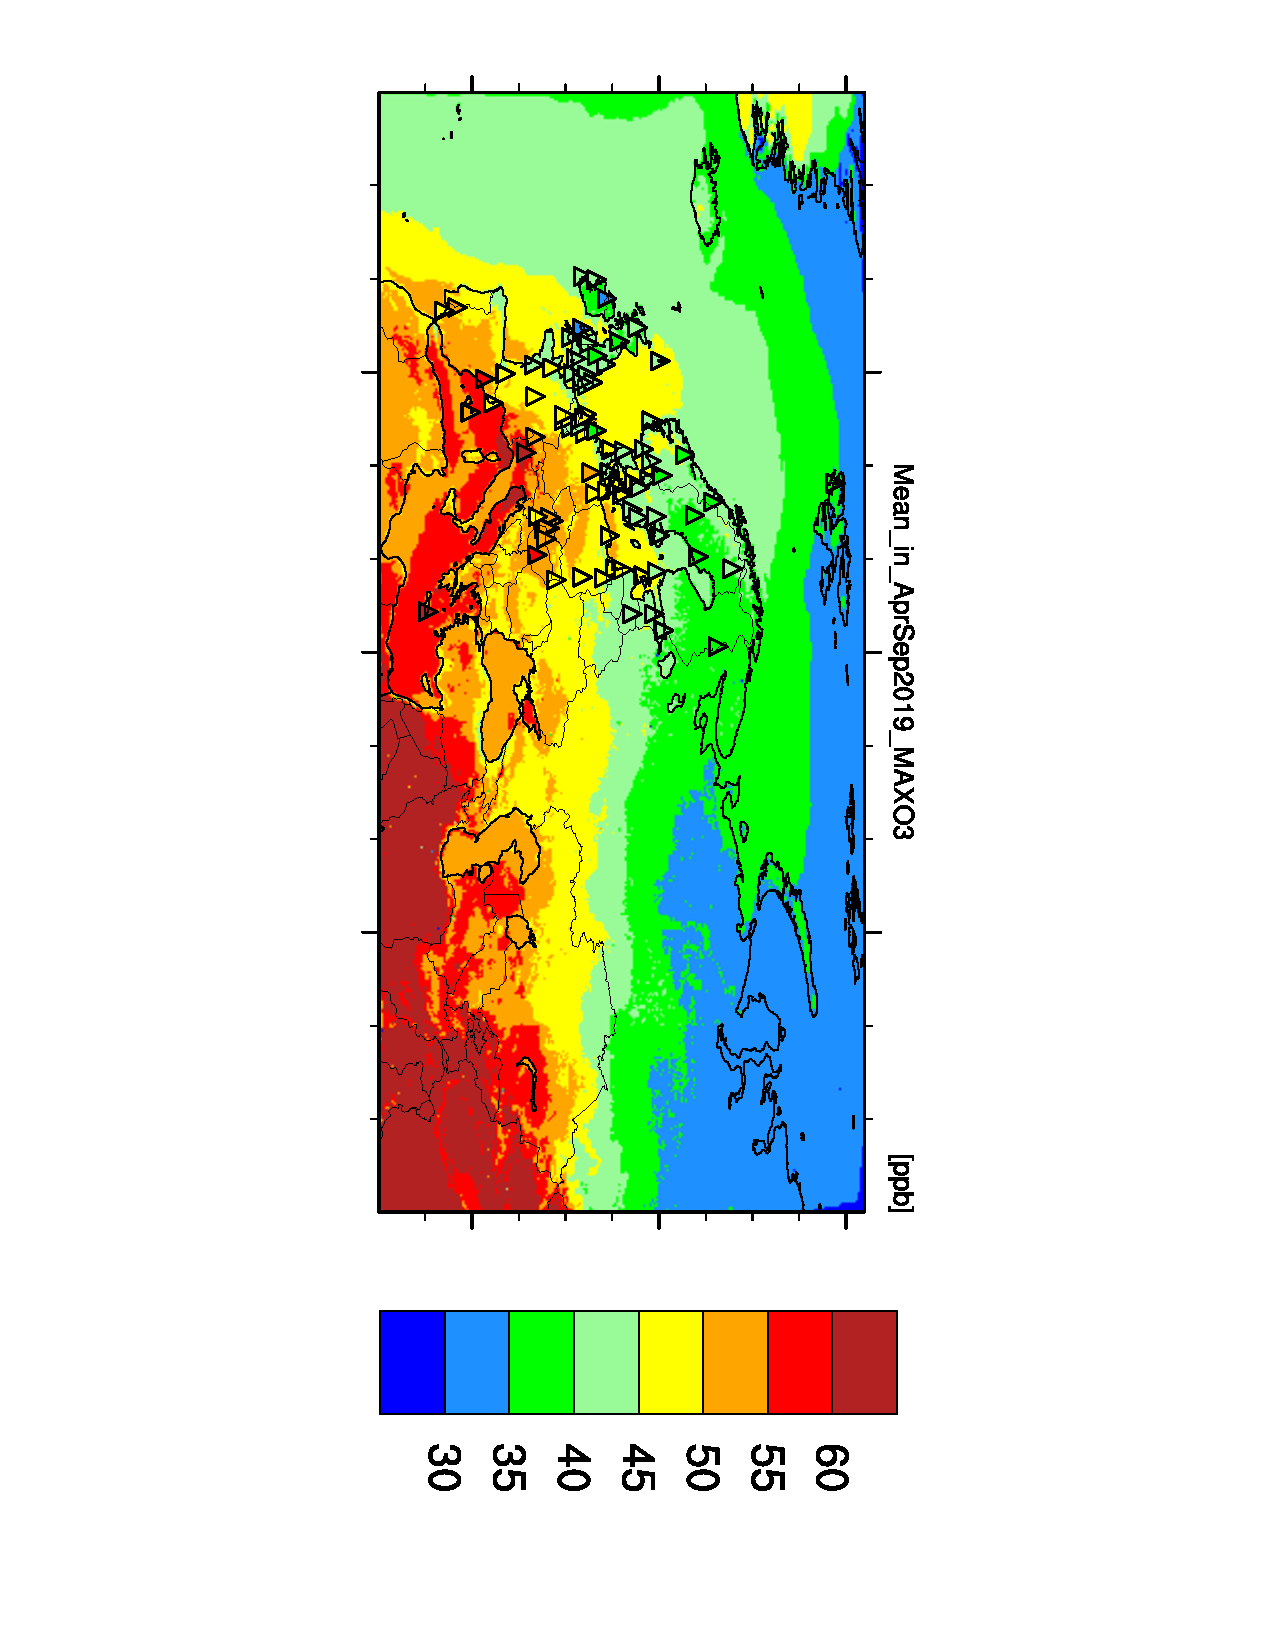
\includegraphics[clip=,angle=90,height=5.5cm,viewport=175 58 420 770]{FIGS_STATUS/MAXO3_AprSep_ModObs_emep_EMEP01.pdf}}
  \subfigure[SOMO35]{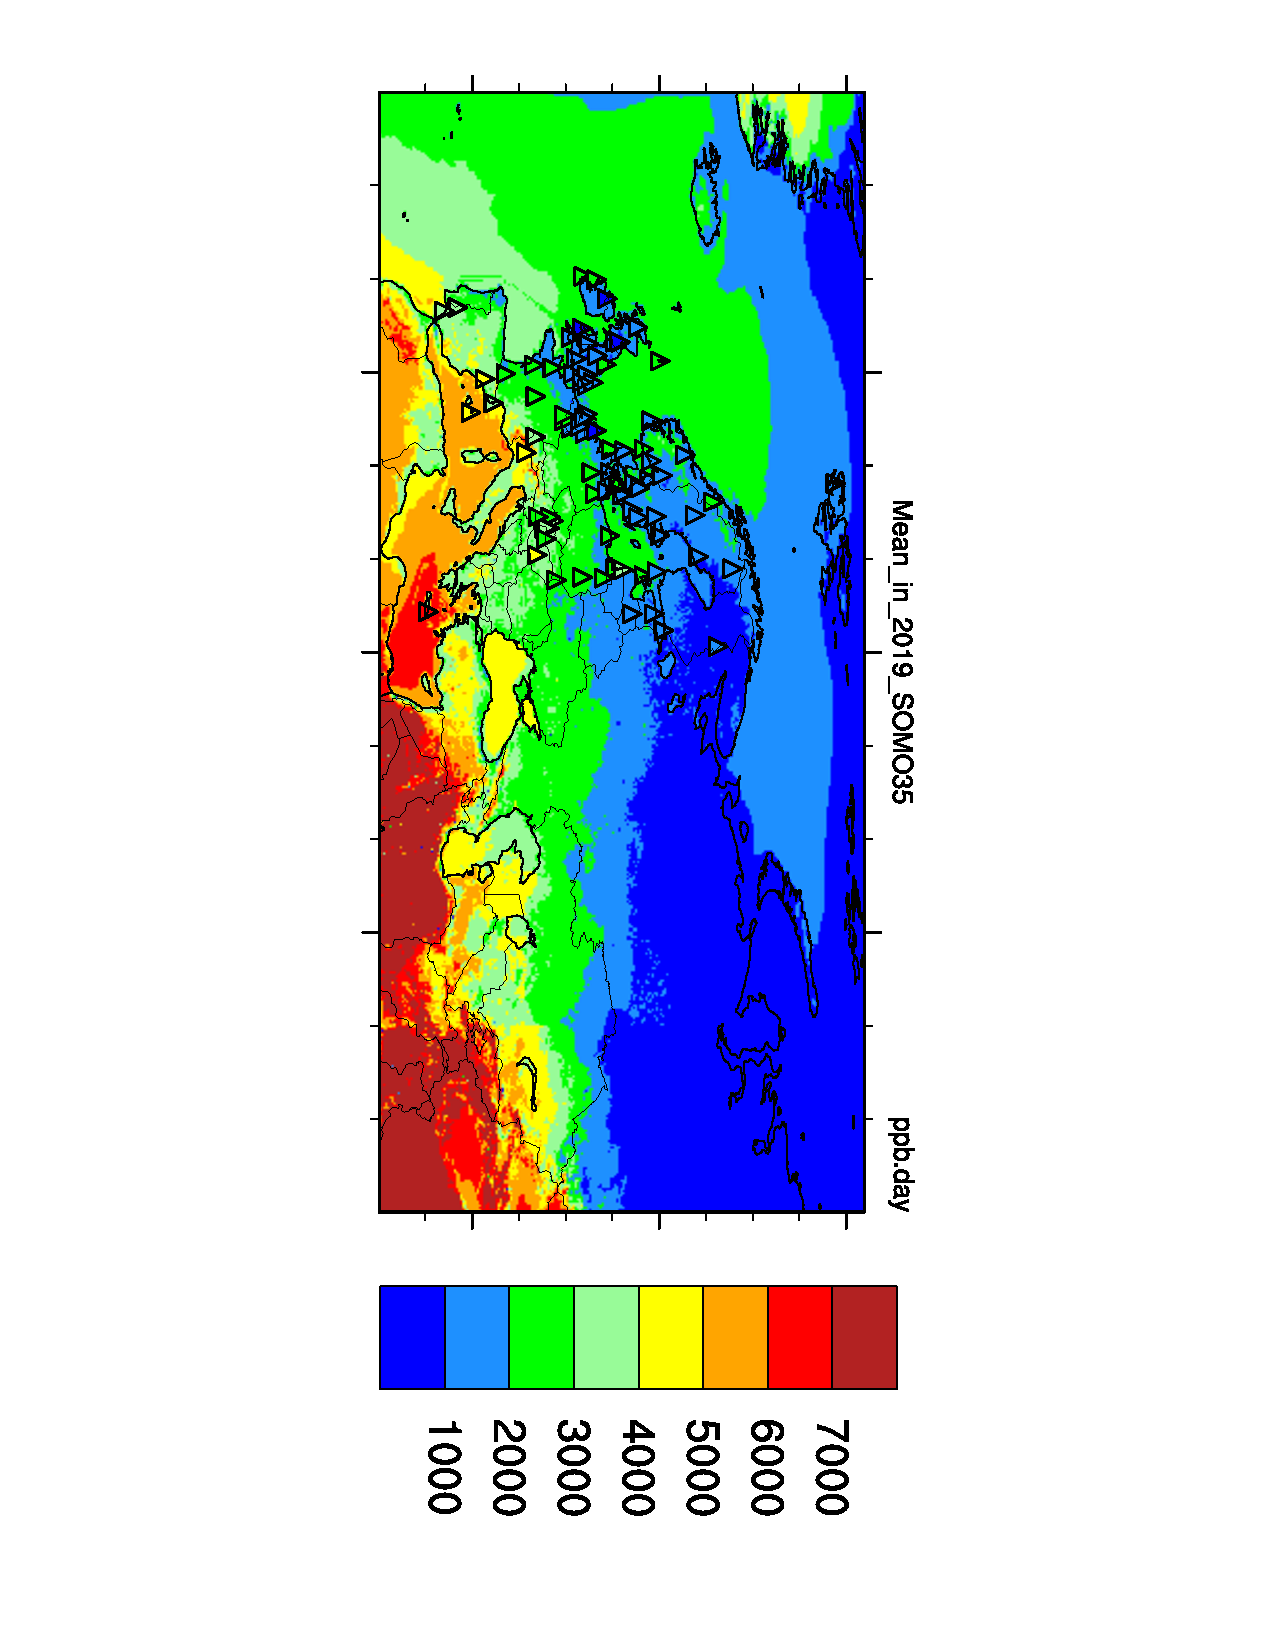
\includegraphics[clip=,angle=90,height=5.5cm,viewport=175 58 420 770]{FIGS_STATUS/SOMO35_ModObs_emep_EMEP01_L20EC.pdf}}
  \subfigure[AOT40]{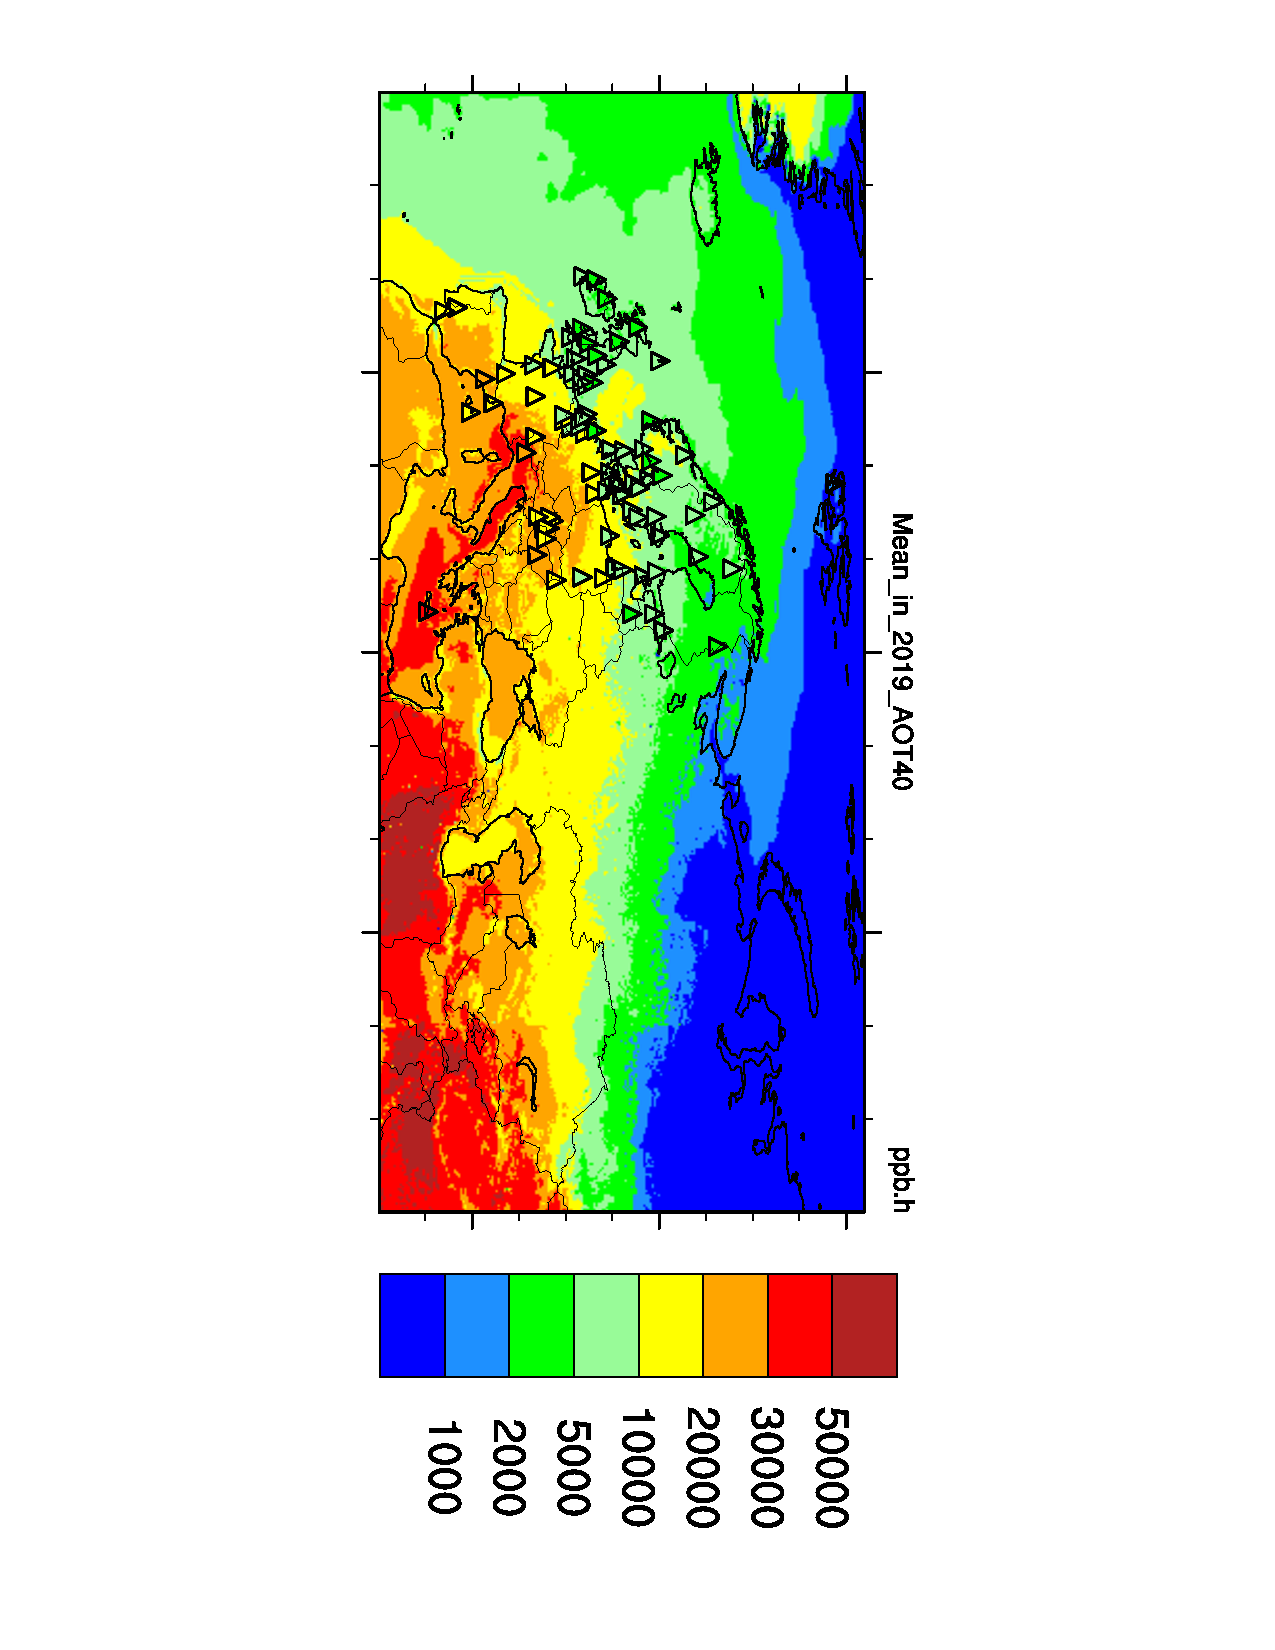
\includegraphics[clip=,angle=90,height=5.5cm,viewport=175 58 420 770]{FIGS_STATUS/AOT40_ModObs_emep_EMEP01_L20EC.pdf}}
\caption{Model results and observations at EMEP stations (triangles) for mean of daily maximum ozone concentrations (a) ([$ppb$], Apr-Sep), SOMO35 (b) [$ppb.d$] and AOT40 for forests (c) [$ppb.h$]. Only data from measurement sites below 500 m a.s.l. are shown.}
\label{fig:indicators_emep}
\end{figure}

The Figures ~\ref{fig:indicators_emep} and ~\ref{fig:indicators_airbase} show a) maxO3 (= mean of the daily max ozone concentration) for the 6-month period April-September, b) SOMO35 (= Sum of Ozone Means Over 35 ppb), c) AOT40 for forests (= Accumulated Ozone exposure over a Threshold of 40 ppb) for the 6-month period April-September using the hours between 08 and 20, and Figure~\ref{fig:indicatorPOD} shows POD$_1$ for forests (= Phytotoxic Ozone Dose above a threshold 1 mmol m$^{-2}$). 

\begin{figure}[H]
  \centering
  \subfigure[maxO3]{\includegraphics[clip=,angle=90,scale=0.60,viewport=187 62 415 750]{FIGS_STATUS/MAXO3_AprSep_ModObs_airbase_EMEP01.pdf}}
  \subfigure[SOMO35]{\includegraphics[clip=,angle=90,scale=0.60,viewport=187 62 415 750]{FIGS_STATUS/SOMO35_ModObs_airbase_EMEP01.pdf}}
  \subfigure[AOT40]{\includegraphics[clip=,angle=90,scale=0.60,viewport=187 62 415 750]{FIGS_STATUS/AOT40_ModObs_airbase_EMEP01_L20EC.pdf}}
\caption{Model results and observations at EEA's e-Reporting stations (triangles) for mean of daily maximum ozone concentrations (a) ([$ppb$], Apr-Sep), SOMO35 (b) [$ppb.d$] and AOT40 for forests (c) [$ppb.h$] in 2018. Only data from measurement sites below 500 m a.s.l. are shown. Urban and traffic stations are not included.}
\label{fig:indicators_airbase}
\end{figure}

These plots indicate good agreement between the modelled and measured ozone metrics in general, although there are indications of a slight underestimation by the model in some areas, most visible for the mean of daily maximum. The number of stations included in EEA's database (Figure~\ref{fig:indicators_airbase}) is, however, so large that it is difficult to see the underlying model fields in some areas.

\begin{figure}[H]
  \centering{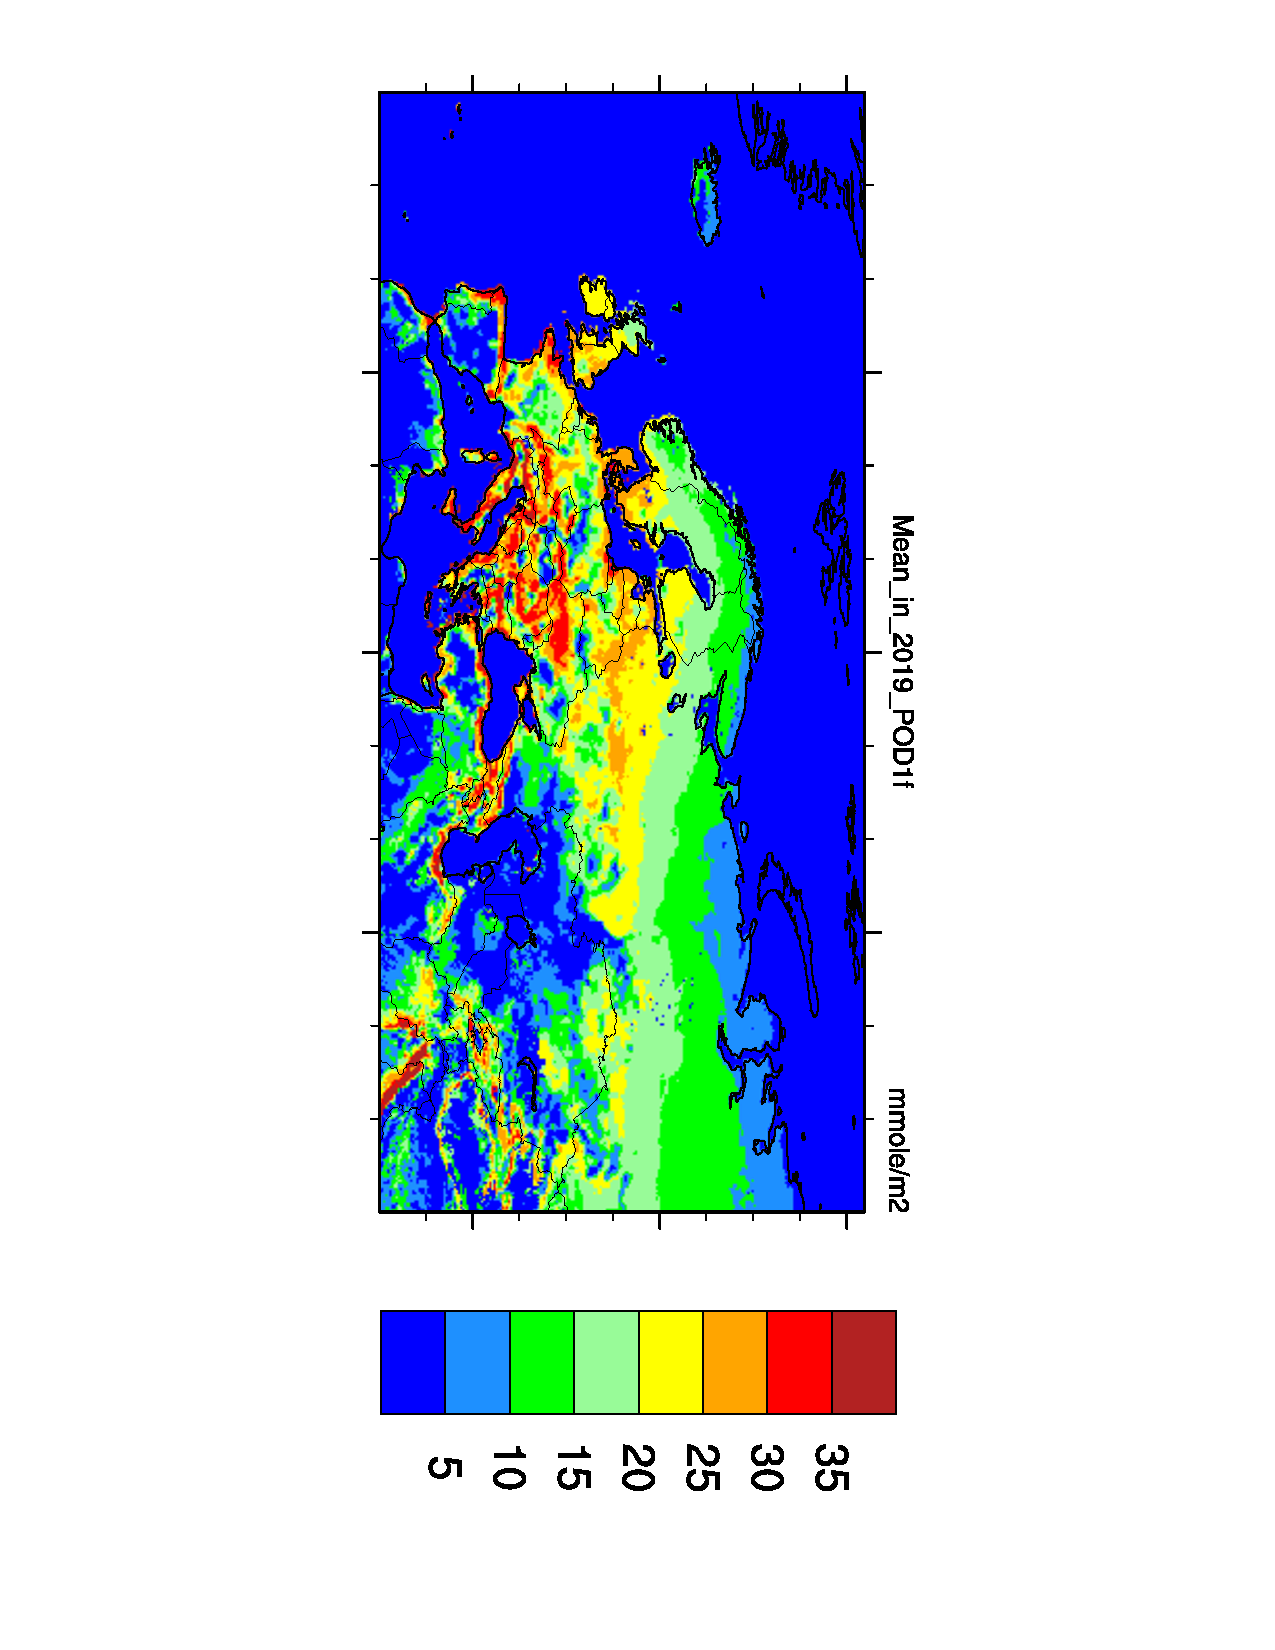
\includegraphics[clip=,angle=90,height=5.5cm,viewport=175 58 420 770]{FIGS_STATUS/POD1f_ModObs_emep_EMEP01.pdf}}
\caption{Model results of POD$_1$ for forests [$mmol m^-2$] in 2018}
\label{fig:indicatorPOD}
\end{figure}

It should be noted that the O$_3$ metrics such as AOT40 are very sensitive to the calculation of vertical O$_3$ gradients between the middle of the surface layer and the 3m height used for comparison with measurements \citep{Tuovinen:EP2007} and thus more difficult to compare with measurement data than, e.g., the mean daily maximum. Indeed, the formulation we use \citep{Simpson_et_al:EMEP} is probably better suited to a lowest model layer of 90m thickness (since we equate the centre of this, ca. 45m, with a `blending-height') than to a lowest model layer of 50m thickness (as used throughout this report). 
The modelled POD$_1$ pattern differs from the other metrics reflecting the influence of additional parameters such as plant physiology, soil moisture etc., and is a metric more indicative of the direct impact of ozone on vegetation than, e.g., AOT40. The POD$_1$ field could, however, not be validated by the EMEP ozone measurement data alone. 

SOMO35 is an indicator for health impacts recommended by WHO, and the results given in Figures~\ref{fig:indicators_emep} and \ref{fig:indicators_airbase} indicate that the health risk associated with surface ozone increased towards southern Europe. Highest levels are seen in the Mediterranean area and Northern Italy. SOMO35 is a health risk indicator without any specific threshold or limit value.

AOT40 and POD$_1$ are indicators for effects on vegetation. UNECE's critical level for forests based on the 6-months AOT40 value is 5000 ppb hours, and the results shown in Figure~\ref{fig:indicators_emep} and Figure~\ref{fig:indicators_airbase} indicate that this level was exceeded in most of Europe in 2018. In parts of central Europe (Germany, Czechia, Switzerland, Austria, etc.) the critical level was exceeded by a very large margin (20000 ppb hours). As discussed in Chapter~\ref{ch:Summer2018} on the 2018 summer heat wave, AOT40 is probably a particularly poor indicator for effects on vegetation in 2018 due to the persistent drought over large areas. During dry periods, plants will reduce or close their stomata as a response to soil water deficit, which in turn will lead to reduced uptake of ozone. Parts of the reason for the elevated atmospheric concentrations of ozone (and the high AOT40 levels) could thus be explained by the reduced uptake in vegetation. 

On the contrary, POD$_1$ takes into account this soil moisture deficit, giving an estimate of the actual flux of ozone into the plants. It is interesting to see the substantial difference in the geographical pattern of AOT40 and POD$_1$ in Figures~\ref{fig:indicators_emep} (c) and \ref{fig:indicatorPOD}. Whereas AOT40 shows a north-south gradient with peak values over southern/central parts of the continent, POD$_1$ is highest along the coast and shows a minimum in central parts of Europe just where high values of AOT40 are seen. This reflects the importance of the soil moisture effect for these two metrics for ozone damage to vegetation. For POD$_1$ the limit value depends on the species and Mills et al (2011) give a value of 4 mmol m$^{-2}$ for birch and beech and 8 mmol m$^{-2}$ for Norway spruce. The results in Figures~\ref{fig:indicators_emep} (c) and \ref{fig:indicatorPOD} indicate that both these limit values were exceeded in most of Europe. The modelled levels of POD$_1$ could, however, not be validated by observations. 

A more detailed comparison between model and measurements for ozone for the year 2018 can be found in \cite{WEB2020:O3}.



%=========================================
\subsection{Particulate matter} 
\label{subs:PMstatus}

Maps of annual mean concentrations of \PM[10] and \PM[2.5] in 2019,
calculated by the EMEP MSC-W model, are presented in
Figure~\ref{fig:PMin2018}. The figures also show annual mean \PM[10]
and \PM[2.5] concentrations observed at the EMEP monitoring network,
represented by colour triangles overlaying the contours of the
modelled concentration fields.

\begin{figure}[H]
  \centering{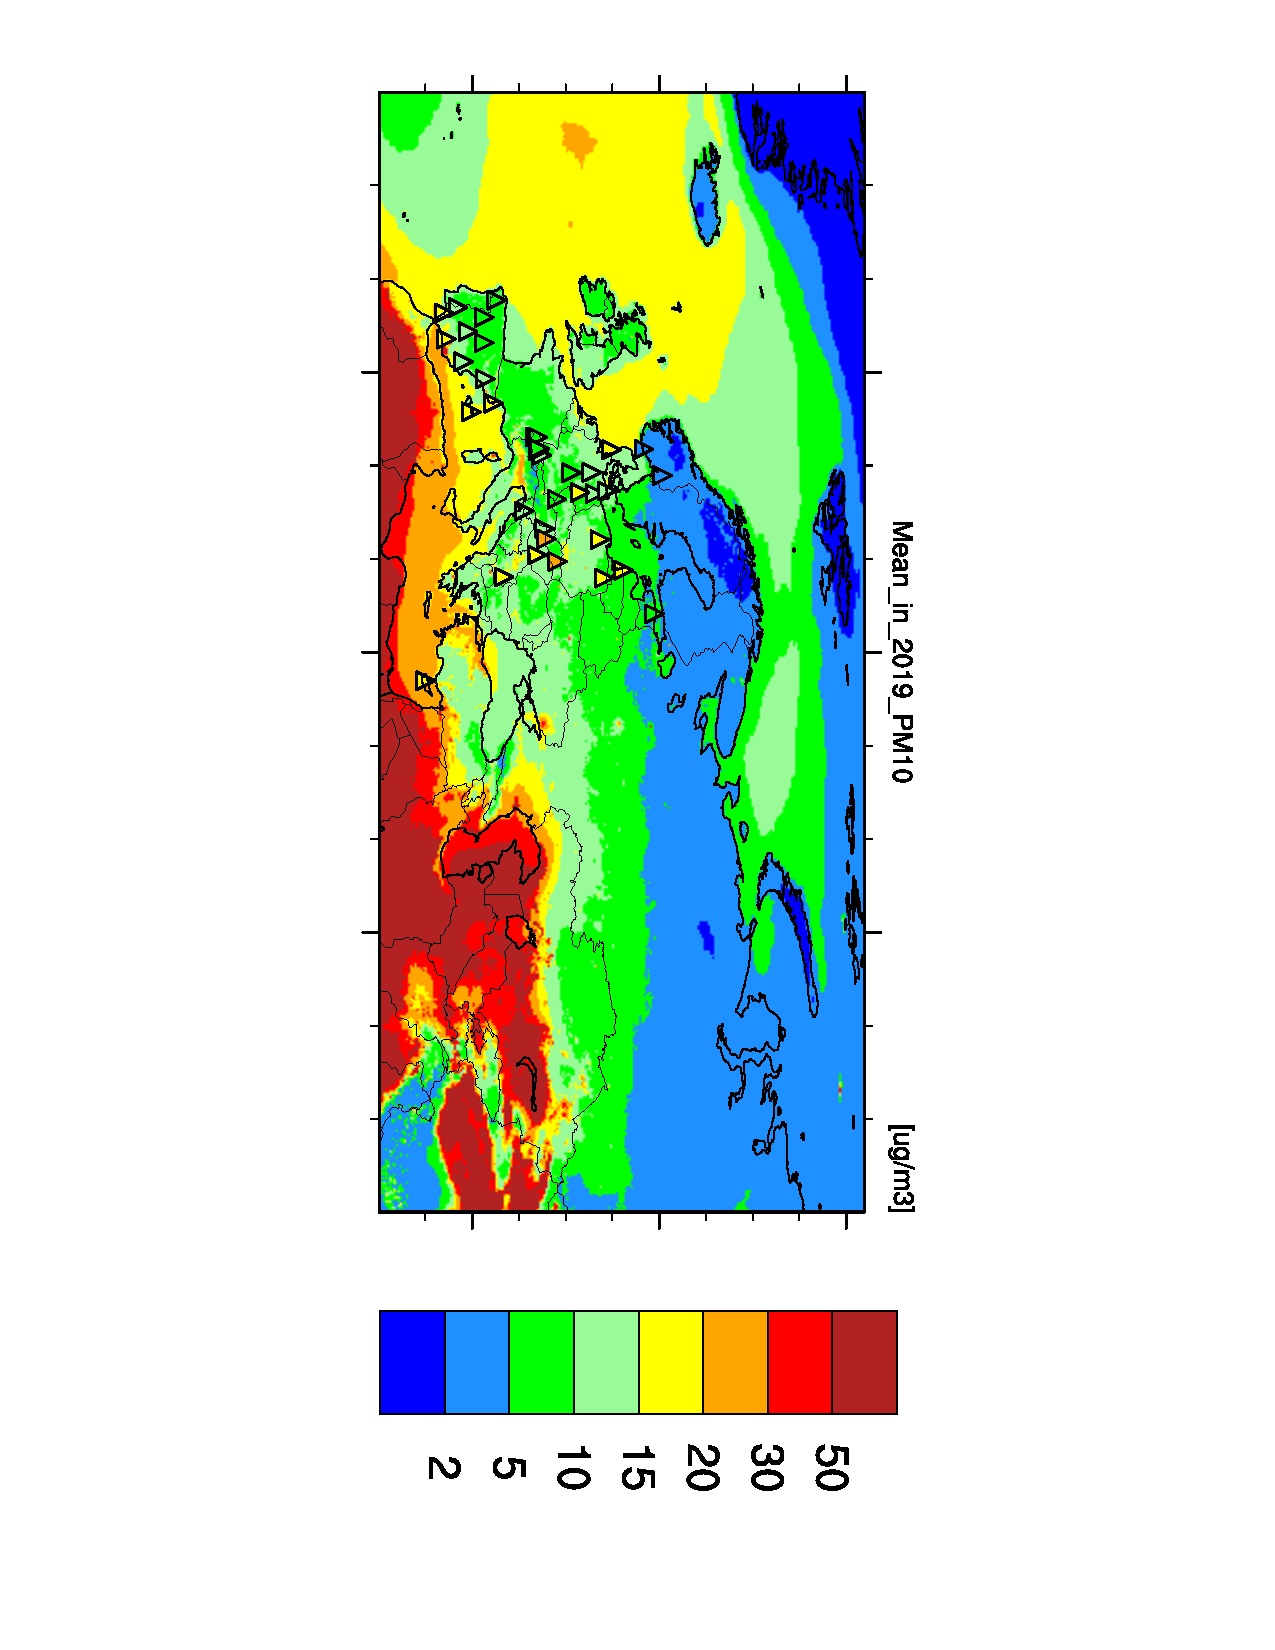
\includegraphics[clip=,angle=90,height=6cm,viewport=175 67 448 754]{FIGS_PM/Mean_in_2019_PM10_EMEP01_ALL.pdf}}\\
  \vspace{0.5cm}
  \centering{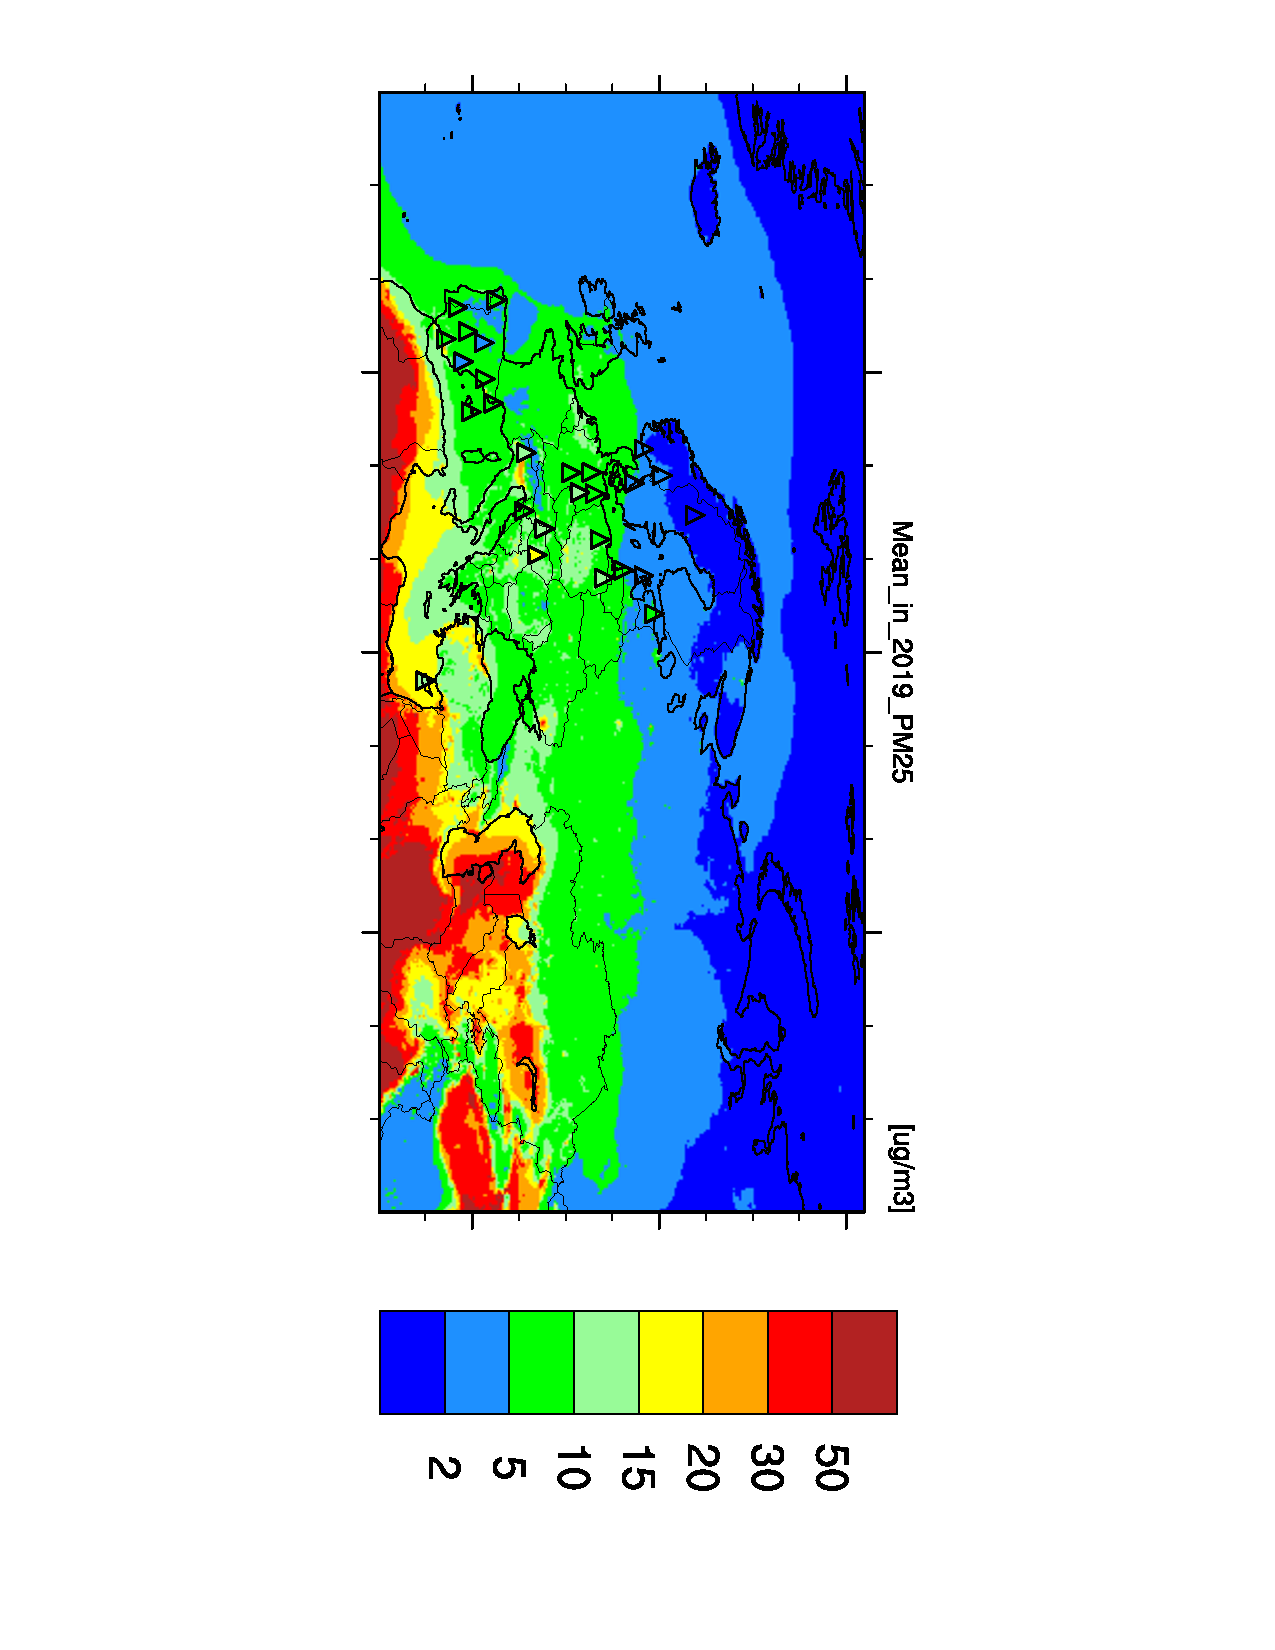
\includegraphics[clip=,angle=90,height=6cm,viewport=175 67 448 754]{FIGS_PM/Mean_in_2019_PM25_EMEP01_ALL.pdf}}
\caption{Annual mean concentrations of \PM[10] and \PM[2.5] in 2019:
  calculated with the EMEP MSC-W model (colour contours) and observed
  at EMEP monitoring network sites (colour triangles). \textit{Note:
    Observations include hourly, daily and weekly data.}}
\label{fig:PMin2018}
\end{figure}


The model results and the observations are well in agreement
regarding the geographical distribution of the annual mean levels of
\PM[10] and \PM[2.5], showing their general increase over land from
north to south. The concentrations are below 2-5 \ug in Northern
Europe, increasing to 5-15 \ug in the mid-latitudes and further south,
with \PM[2.5] levels being somewhat lower than those of
\PM[10]. Figure~\ref{fig:PMin2018} displays fairly homogeneous levels
of regional background PM over most of Central and Western Europe,
with somewhat elevated \PM[10] levels of 15-20 \ug in the Po Valley and
the Benelux. The observations also show elevated \PM[10] concentrations in Poland, Czechia and Hungary, while
the model calculates high PM for the regions east of the Caspian Sea
(parts of Kazakhstan, Uzbekistan, Turkmenistan) and over the southern
Mediterranean, with annual mean concentrations in excess of 50
\ug. As explained in earlier EMEP reports, these high PM
concentrations are due to windblown dust from the arid soils and
deserts of Central Asia, though the accurateness of the calculated
values still cannot be verified due to the lack of
observations in these regions.

There is good agreement between the modelled and observed
distributions of annual mean \PM[10] and \PM[2.5], with correlation
coefficients of 0.66 and 0.81, respectively. Overall, the model
underestimates the observed annual mean of \PM[10] by 22\% and
\PM[2.5] by 14\%. A comprehensive model evaluation is provided in~\cite{WEB2020:PM}.

In terms of meteorological conditions, the year 2018 was relatively warm across the EMEP area (except for Asian parts of Russia and Kazakhstan), particularly in Central Europe  (Figure~\ref{fig:2018-avMET}). The spring and summer were also notably warm in Fennoscandia, the Baltic countries and Eastern Europe. Mild winter conditions would mean less need for residential heating, resulting in lower emissions from this sector. Moreover, stagnant air conditions (with temperature inversion, low wind speed and thin mixing layer), causing elevated pollution levels, are less frequent in warm winters. In spring/summer time, higher temperatures would enhance evaporation of semi-volatile inorganic and organic aerosols (SIA and SOA), though the more efficient oxidation contributes to secondary aerosol formation. Furthermore, in Northern and Central Europe, the Baltic region and European Russia, the year 2018 was dry compared to the 2000-2017 average, especially in the spring and summer, which contributed to the photochemistry and secondary aerosol formation. On the other hand, it was a relatively wet year in Western and Southern Europe (Figure~\ref{fig:2018-avMET}) and also in parts of Central, Northern and Eastern Europe in the winter~\citep{CAMS2019}, so that the pollutants were more efficiently removed from the air in those regions.  

%\begin{figure}[H]
%  \centering{\includegraphics[clip=,angle=90,height=3cm,viewport=175 67 448 754]{FIGS_PM/RelAnomaly_PM10_2018_vs_2000-2017.pdf}}
%  \centering{\includegraphics[clip=,angle=90,height=3cm,viewport=175 67 448 754]{FIGS_PM/RelAnomaly_PM25_2018_vs_2000-2017.pdf}}
%\caption{Relative anomalies of mean \PM[10] and \PM[2.5] in 2018 from the 2000-2017 mean.}
%\label{fig:PManomin2018}
%\end{figure}

Figure~\ref{fig:PManomin2018} presents the relative anomalies of mean \PM[10] and \PM[2.5] concentrations in 2018 relative to 2000-2017 averages simulated with a model version used for 2019 reporting and EMEP reported emissions. It shows that the PM pollution levels in 2018 were rather moderate, in particular in Central, Western and Southern Europe (10-30\% lower compared to the 18-year average). Only in Turkey, the Caucasus region, Ukraine, the Baltic countries and southern parts of Finland and Sweden, \PM[10] and \PM[2.5] levels were higher. The prolonged heat wave affected Central and Northern Europe during summer 2018 and caused enhanced aerosol levels; this is discussed in Chapter \ref{ch:Summer2018}.


\subsubsection[PM exceedances]{Exceedances of EU limit values and WHO Air Quality Guidelines in 2018}
\label{subsec:PMexc}

In this section we compare \PM[10] and \PM[2.5] exceedances
of EU critical limits and WHO recommended Air Quality
Guidelines \citep{WHO:AQG}, calculated by the EMEP MSC-W model, with
those measured at EMEP sites. The EU limit values for \PM[10] (Council
Directive 1999/30/EC) are 40 \ug for the annual mean and 50 \ug for
the daily mean concentrations, with the daily limit not to be exceeded
more than 35 times per calendar year~\citep{EU2008}. For \PM[2.5], the
annual mean limit value of 25 \ug entered into force on 01.01.2015.

The Air Quality Guidelines (AQG) recommended by WHO \citep{WHO:AQG}
are:
\begin{itemize}
\item for \PM[10]: 20 \ug annual mean, 50 \ug 24-hourly (99th perc. or 3 days per year)
\item for \PM[2.5]: 10 \ug annual mean, 25 \ug 24-hourly (99th perc. or 3 days per year)
\end{itemize}


The EU limit values for protection of human health from particulate
matter pollution and the WHO AQG for PM should apply to concentrations
for zones or agglomerations, in rural and urban areas,
which are representative for exposure of the general
population. \PM[10] and \PM[2.5] concentrations calculated with the
EMEP MSC-W model on the 0.1$\degrees \times$ 0.1$\degrees$ grid cannot
reproduce urban hotspot levels, but give a reasonable representation
of PM levels occurring in rural and, to some extend, in urban background
areas.


Model results and EMEP observational data show that the annual mean \PM[10] concentrations were below the EU limit value of 40 \ug for all of Europe in 2018 (Figure~\ref{fig:PMin2018}). The model calculates annual mean \PM[10] above the WHO recommended AQG of 20 \ug
in only small regions in the Po Valley and western Turkey. The highest
observed annual mean \PM[10] concentrations, exceeding the AQG of 20 \ug, were registered in Slovakia (SK0007) with 26 \ug, Greece (GR0001, but only 53\% data coverage) with 25 \ug, in Cyprus (CY0002) with 24 \ug, in Czechia (CZ0003) with 23 \ug, the Netherlands (NL0010R) with 21 \ug and Hungary (HU0002) with 20 \ug. Further, the observations and model results show that annual mean \PM[2.5] concentrations (Figure~\ref{fig:PMin2018}) in 2018 were below the EU limit value of 25 \ug (except in the Po Valley according to the model). However, there were observed cases of exceedance of the WHO AQG value of 10 \ug by annual mean \PM[2.5] at seventeen sites, with the highest values in Hungary (HU0003 with 16 \ug and HU0002 with
15.5 \ug) and in Austria (AT0002) and Czechia (CZ0003) both with 14.5 \ug.


%\begin{figure}[ht]
%  \centering{\includegraphics[clip=,angle=90,height=6cm,viewport=180 67 440 754]{FIGS_PM/ExcDays_PM10_ModObs_EMEP01_2018.pdf}}\\
%  \vspace{0.5cm}
%  \centering{\includegraphics[clip=,angle=90,height=6cm,viewport=180 67 440 754]{FIGS_PM/ExcDays_PM25_ModObs_EMEP01_2018.pdf}}
%\caption{Calculated (with 0.1\degrees resolution) and observed (triangles) number of days with
%  exceedances in 2018: \PM[10] exceeding 50 \ug (upper) and \PM[2.5]
%  exceeding 25 \ug (lower panel). \textit{Note: The EU Directive requires no
%    more than 35 days with exceedances for \PM[10], whereas WHO
%    recommends no more than 3 days with exceedances for \PM[10] and
%    \PM[2.5] per calendar year. }}
%\label{fig:PMexceed}
%\end{figure}


The maps in Figure~\ref{fig:PMexceed} show the number of days with
exceedances of 50 \ug for \PM[10] and 25 \ug for \PM[2.5] in 2018:
modelled values as colour contours and observed values as triangles.

Out of the 62 sites with daily or hourly \PM[10] measurements with data
coverage above 75\%, exceedance days were observed at 36 sites. No
violations of the \PM[10] EU limit value (more than 35 exceedance
days) were observed. Still, 18 sites had more than 3 exceedance days
(according to WHO AQG recommendations). The highest numbers of days
with observed exceedances of \PM[10] were 25 at CY0002 and SK0007, and 17
at CZ0003.

\PM[2.5] concentrations exceeded the WHO AQG value at 31 out of 41
stations in 2018. Among those, at 21 sites the number of exceedance
days were more than 3 (the recommended limit according to WHO AQG). 
The highest number of exceedance days registered were 50, which were observed at HU0002, IT0004 and PL0009, followed by 49 and 48 exceedance days at AT0002 and HU0003, respectively.

The modelled numbers of exceedance days in 2018 show in general a good correspondence with the observations, with somewhat better agreement for \PM[10] than for \PM[2.5]. For \PM[10], the model underestimates the frequency of exceedances of the EU limit value of 50 \ug for some central European sites, for instance at SK0007 and CZ0003 (no modelled exceedance days versus, respectively, 25 and 17 observed), PL0009 (1 exceedance day vs. 11 observed) and HU0002 (no exceedance day vs. 10 observed). On the other hand, the model tends to somewhat overestimate the number of exceedance days at some Mediterranean sites, influenced by Saharan dust, e.g. at the Cypriot site CY0002 (28 vs. 25 observed) and several Spanish sites (in particular ES0007 with 23 vs. 5 observed). Practically all the exceedances registered at the central European sites occurred during winter and autumn (and also in spring at e.g. Polish, Dutch, and Hungarian sites). By contrast, at the Mediterranean sites the exceedances were more frequent during summer.

For \PM[2.5], the model calculates 17 exceedance days versus 50 observed at PL0009, 28 versus 49 observed at AT0002, 17 versus 48 observed at HU0003. At the Dutch sites, the model slightly underestimates observed \PM[2.5] exceedance days at NL0009, but overestimates those at NL0010, NL0091 and NL0644. Also, the numbers of exceedance days are overestimated by the model at the Croatian site HR0002 (39 vs 2 observed) and at Ispra in Italy (IT0004, 64 vs 49 observed). As for \PM[10], the model calculates a larger number of exceedance days for \PM[2.5] compared with observations at CY0002 and several Spanish sites, which is related to the uncertainties in windblown dust modelling. The seasonality of \PM[2.5] exceedances is similar to that of \PM[10], with most exceedance days at the Mediterranean sites in summer and at the other sites in winter, spring and autumn. The only difference is that the largest number of \PM[2.5] exceedances at three of four German sites occurred in spring, while much fewer occurred during the cold seasons.

%\clearpage
\begin{figure}[H]
  \centering
  \subfigure[oxidized S] {\includegraphics*[viewport=187 62 415 750,clip,angle=90,scale=0.60]{FIGS_STATUS/Mean_in_2018_DEP_SOX_EMEP01.pdf}}
  \subfigure[oxidized N] {\includegraphics*[viewport=187 62 415 750,clip,angle=90,scale=0.60]{FIGS_STATUS/Mean_in_2018_DEP_OXN_EMEP01.pdf}}
  \subfigure[Reduced N] {\includegraphics*[viewport=187 62 415 750,clip,angle=90,scale=0.60]{FIGS_STATUS/Mean_in_2018_DEP_RDN_EMEP01.pdf}} 
 \caption{Deposition of sulphur and nitrogen [mg(S)m$^{-2}$, mg(N)m$^{-2}$] in 2018.}
\label{deps}
\end{figure}


\subsection{Deposition of sulphur and nitrogen} %Hilde to rewrite. Anna to update figures
\label{subs:dep}

Modelled total depositions of sulphur and oxidised and reduced nitrogen are presented in Figure \ref{deps}.
For sulphur, many hot spots are found in the south-eastern part of the domain. In addition, volcanic emissions of SO$_2$ lead to high depositions in and around Sicily.

Oxidised nitrogen depositions are highest in northern Germany, the Netherlands, Belgium, Poland and northern Italy. These countries also have high depositions of reduced nitrogen, as do parts of the United Kingdom, France, Belgium in western Europe, and Turkey, Georgia, Armenia, Azerbaijan, Kyrgyzstan, Uzbekistan and Tajikistan in the east. 

In Figure \ref{wdeps} wet depositions of nitrogen and sulphur compounds are compared to measurements at EMEP sites for 2018. Overall, the bias of the model with respect to measurements is around 
-36\% to +5\%, but higher for individual sites. A more detailed comparison between model and measurements for the year 2018 can be found in \cite{WEB2020:SN}.

\begin{figure}[H]
  \centering
  \subfigure[oxidized S] {\includegraphics*[viewport=187 62 415 750,clip,angle=90,scale=0.60]{FIGS_STATUS/so4wdep_2018_ModObs_EMEP01.pdf}}
  \subfigure[oxidized N] {\includegraphics*[viewport=187 62 415 750,clip,angle=90,scale=0.60]{FIGS_STATUS/no3wdep_2018_ModObs_EMEP01.pdf}}
   \subfigure[Reduced N] {\includegraphics*[viewport=187 62 415 750,clip,angle=90,scale=0.60]{FIGS_STATUS/nhxwdep_2018_ModObs_EMEP01.pdf}} 
 \caption{Modelled wet deposition of sulphur and nitrogen [mg(S)m$^{-2}$, mg(N)m$^{-2}$] in 2018, with EMEP observations on top (marked by triangles).}
\label{wdeps}
\end{figure}

\subsection{Exceedances of critical loads of acidification and eutrophication}\label{subs:exceedSnN}

The exceedances of European critical loads (CLs) are computed for the total nitrogen
(N) and sulphur (S) depositions modelled on the 0.1$\degrees \times$ 0.1$\degrees$
longitude-latitude grid (approx. 11 x 5.5 km$^{2}$ at 60$\degrees$N).
Exceedances are calculated for the European critical loads documented in \cite{Hettelingh:2017}, while
a description of the methods is given in \cite{DeVries:2015}. The
critical loads data for eutrophication by N (CL eut N) and for acidification by N and S
(CL acid) are also used by the EMEP Centre CIAM (located at IIASA) in their integrated assessment
modelling. The exceedance in a grid cell is the so-called ’average accumulated
exceedance’ (AAE), which is calculated as the area-weighted average of the
exceedances of the critical loads of all ecosystems in this grid cell. The units for
critical loads and their exceedances are equivalents (eq; same as \textit{moles of charge},
molc) per area and time, making S and N depositions comparable on their impacts, which is important for
acidity CLs.

Critical loads are available for about 4 million ecosystems in Europe covering an area
of about 3 million km$^{2}$ (west of 42$\degrees$E). The exceedances (AAE) of those critical loads
are computed on a 0.1$\degrees \times$ 0.1$\degrees$ longitude-latitude grid, and maps for the deposition in
the years 2017 and 2018 are shown in Figures \ref{fig:eutN} and \ref{fig:acid}. As it can be seen from
the maps, critical loads for eutrophication are exceeded in practically all countries in
both years. The exceedance occurs on 63.3\% (2017) and 64.8\% (2018) of the
ecosystem area. European average AAE is about 281 eq ha$^{-1}$ yr$^{-1}$ (2017) and 273 eq
ha$^{-1}$ yr$^{-1}$ (2018). The highest exceedances of CLs are found in the Po Valley in Italy, the
Dutch-German-Danish border areas and in north-eastern Spain.
By contrast, critical loads of acidity are exceeded in a much smaller area. Hot spots of
exceedances can be found in the Netherlands and its border areas to Germany and
Belgium, and some smaller maxima in southern Germany and Czechia,
whereas most of Europe is not exceeded (grey areas). Acidity exceedances occur
on 5.5\% (2017) and 5.2\% (2018) of the ecosystem area, and the European average
AAE is about 34 eq ha$^{-1}$ yr$^{-1}$ (2017) and 24 eq ha$^{-1}$ yr$^{-1}$ (2018).

\begin{figure}[ht]
  \centering
  \subfigure{\includegraphics*[scale=0.35]{FIGS_STATUS/CL_Ex_eutN_2017.png}}
  \subfigure{\includegraphics*[scale=0.35]{FIGS_STATUS/CL_Ex_eutN_2018.png}}
 \caption{Exceedance of Critical Load for Eutrophication for the Year 2017 (left) and 2018 (right).}
\label{fig:eutN}
\end{figure}

\begin{figure}[ht]
  \centering
  \subfigure{\includegraphics*[scale=0.35]{FIGS_STATUS/CL_Ex_acid_2017.png}}
  \subfigure{\includegraphics*[scale=0.35]{FIGS_STATUS/CL_Ex_acid_2018.png}}
 \caption{Exceedance of Critical Load for Acidification for the Year 2017 (left) and 2018 (right).}
\label{fig:acid}
\end{figure}

\clearpage
\bibliographystyle{copernicus}         % change bibliography-name after each
\renewcommand\bibname{References}      % bibliographystyle command!
\addcontentsline{toc}{section}{References}
\bibliography{Refs,EMEP_Reports,RefsMeteo,RefStatusPM}
